\documentclass[main.tex]{subfiles}

\begin{document}
\subsection{Explain how decision problems can be formalized by the notion of language of finite words. Develop an example of a language that formalizes a problem}
\emph{cf : \cite{2018}}

First, we need to define these concepts :
\par\textit{Decision problems :} the set of inputs for which the answer is yes.
    In other words, an instance of a decision problem is whether or not
an input A is part of the solution package. It is important to distinguish
between an instance and a problem (the former refers to a specific input whereas the
second takes as a reference all possible inputs).
\par\textit{Language of finite words:} The language of an M machine is defined as : L(M) = A. If A is the set
of all the words (strings) that the M machine accepts.
We can say that:
\begin{itemize}
    \item M accepts A
    \item M recognizes A
\end{itemize}

\todo[inline]{add examples}

\subsection{Define the notion of configuration of a Turing machine. Define the notion of computation of a deterministic Turing machine M on a word $w$.}
%Renato - 25/12
%NOT FINISHED
\emph{cf Sipser, pp. 140-141}

A \emph{configuration} of a TM consists of three items --- the current state, tape contents 
and head location. For a state $q$ and two strings $u$ and $v$ over the tape alphabet $\Gamma$ we could write a configuration $uqv$ where : $uv$ is the current content of the tape,
$q$ is the current state and the head location is the first symbol of $v$.

$1011q_701111$ represents a configuration when the tape is $101101111$, the current state is $q_7$ and the head is on the second $0$ (given by the position of $q_7$ in $1011q_701111$.)


\subsection{Are nondeterministic Turing machines more powerful than deterministic Turing machines as deciders ?Justify your answer by proving that every nondeterministic Turing machine has an equivalent deterministic Turing machine}
\emph{cf Sipser, pp. 150}

A nondeterministic Turing machine is defined in the expected way. At any point
in a computation the machine may proceed according to several possibilities.
The transition function for a nondeterministic Turing machine has the form
\todo[inline]{add equation}
\par The computation of a nondeterministic Turing machine is a tree whose branches
correspond to different possibilities for the machine. \todo[inline]{add schema}
If some branch of the computation leads to the accept state, the machine accepts its input. 
\par Now we show that nondeterminism does not affect the power of the Turing machine model. 
\par\rule{\textwidth}{0.4pt}
\textbf{THEOREM 3.16} \textit{Every nondeterministic Turing machine has an equivalent deterministic Turing
machine.}
\par\textbf{PROOF IDEA} We can simulate any nondeterministic TM N with a deterministic TM D. The idea behind the simulation is to have D try all possible branches
of N’s nondeterministic computation. If D ever finds the accept state on one of
these branches, D accepts. Otherwise, D’s simulation will not terminate.
We view N’s computation on an input w as a tree. Each branch of the tree
represents one of the branches of the nondeterminism. Each node of the tree
is a configuration of N. The root of the tree is the start configuration. The
TM D searches this tree for an accepting configuration. Conducting this search
carefully is crucial lest D fail to visit the entire tree. A tempting, though bad,
idea is to have D explore the tree by using depth-first search. The depth-first
search strategy goes all the way down one branch before backing up to explore
other branches. If D were to explore the tree in this manner, D could go forever
down one infinite branch and miss an accepting configuration on some other
branch. Hence we design D to explore the tree by using breadth first search
instead. This strategy explores all branches to the same depth before going on
to explore any branch to the next depth. This method guarantees that D will
visit every node in the tree until it encounters an accepting configuration. 
\par\textbf{PROOF } The simulating deterministic TM D has three tapes. By Theorem 3.13 this arrangement is equivalent to having a single tape. The machine D
uses its three tapes in a particular way, as illustrated in the following figure. Tape
1 always contains the input string and is never altered. Tape 2 maintains a copy
of N’s tape on some branch of its nondeterministic computation. Tape 3 keeps
track of D’s location in N’s nondeterministic computation tree.
\begin{center}
    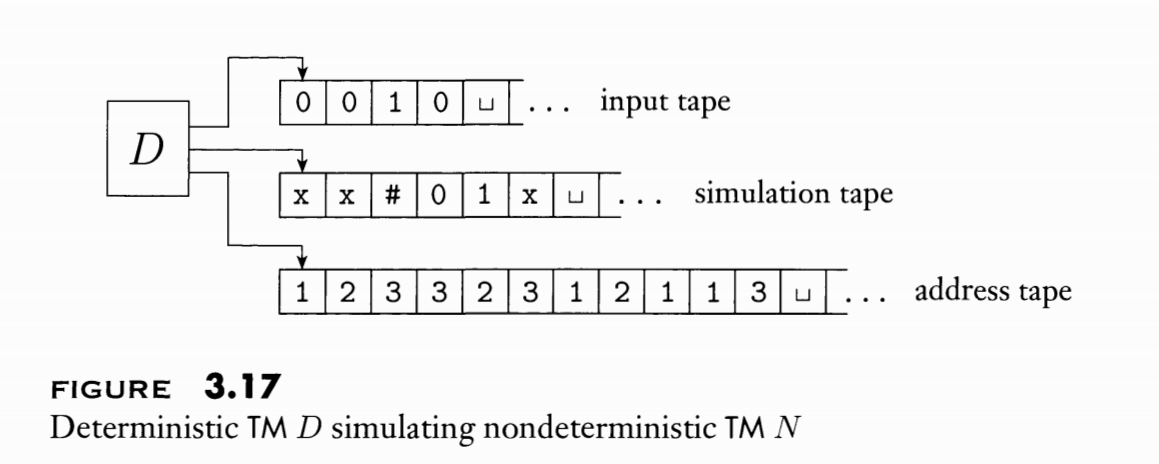
\includegraphics[scale=0.47]{images/figure317.png}
\end{center}
Let’s first consider the data representation on tape 3. Every node in the tree
can have at most \textit{b} children, where b is the size of the largest set of possible
choices given by \textit{N’}s transition function. To every node in the tree we assign an
address that is a string over the alphabet $\sum_{b}$ = \{1, 2, ..., b\}. We assign the address 231 to the node we arrive at by starting at the root, going to its 2nd child,
going to that node’s 3rd child, and finally going to that node’s lst child. Each
symbol in the string tells us which choice to make next when simulating a step in
one branch in N’s nondeterministic computation. Sometimes a symbol may not
correspond to any choice if too few choices are available for a configuration. In
that case the address is invalid and doesn’t correspond to any node. Tape 3 contains a string over . It represents the branch of N’s computation from the root
to the node addressed by that string, unless the address is invalid. The empty
string is the address of the root of the tree. Now we are ready to describe D.
\begin{enumerate}[label=\textbf{\arabic*}]
    \item Initially tape 1 contains the input $w$, and tapes 2 and 3 are empty.
    \item Copy tape 1 to tape 2.
    \item Use tape 2 to simulate N with input $w$ on one branch of its nondeterministic computation. Before each step of N consult the next symbol on tape 3
to determine which choice to make among those allowed by N’s transition
function. If no more symbols remain on tape 3 or if this nondeterministic
choice is invalid, abort this branch by going to stage 4. Also go to stage 4
if a rejecting configuration is encountered. If an accepting configuration is
encountered, accept the input.
    \item Replace the string on tape 3 with the lexicographically next string. Simulate the next branch of N’s computation by going to stage 2. 
\end{enumerate}

\subsection{Given a Turing machine $M$ and a word $w$, give the computation of $M$ on $w$. Does $M$ accept $w$}
\emph{cf Sipser, pp. 141}


The start configuration of $M$  on input $w$ is the configuration $q_0$ $w$, which
indicates that the machine is in the start state $q_0$ with its head at the leftmost
position on the tape. In an accepting configuration the state of the configuration
is $q_{accept}$. In a rejecting configuration the state of the configuration is $q_{reject}$.
Accepting and rejecting configurations are halting configurations and do not
yield further configurations. Because the machine is defined to halt when in the
states $q_{accept}$ and $q_{reject}$, we equivalently could have defined the transition function to have the more complicated form \todo[inline]{add equation}
where Q’ is Q
without $q_{accept}$ and $q_{reject}$.
\begin{center}
    \rule{0.3\textwidth}{0.4pt}
\end{center}
\par A Turing machine $M$ \textbf{accepts} input $w$ if a sequence of configurations $C_{1},C_{2}, ..., C_{k}$ exists, where
\begin{enumerate}[label=\textbf{\arabic*}]
    \item $C_{1}$ is the start configuration of $M$ on input $w$
    \item each $C_{i}$ yields $C_{i+1}$, and
    \item $C_{k}$ is an accepting configuration
\end{enumerate}
 
\subsection{Define when a Turing machine recognizes a language $L$ and when it decides a language $L$. What is the fundamental difference between those two notions ? Why do we use deciders to formalize the intuitive notion of algorithm}
\emph{cf Sipser, pp. 142}

The collection of strings that $M$ accepts is the language of $M$, or the language recognized by $M$, denoted $L(M)$. 
\begin{mytheo*}{}
Call a language Turing-recognizable if some Turing machine
recognizes it.
\end{mytheo*}


When we start a Turing machine on an input, three outcomes are possible.
The machine may accept, reject, or loop. By loop we mean that the machine simply
does not halt. Looping may entail any simple or complex behaviour that never
leads to a halting state.
A Turing machine M can fail to accept an input by entering the $q_{reject}$ state
and rejecting, or by looping. Sometimes distinguishing a machine that is looping
from one that is merely taking a long time is difficult. 
\par For this reason we prefer Turing machines that halt on all inputs; such machines never loop. These machines are called deciders because they always make a decision to accept or reject.
A decider that recognizes some language also is said to decide that language. 
\begin{mytheo*}{}
Call a language Turing-decidable or simply decidable if some
Turing machine decides it.
\end{mytheo*}

\subsection{Define the notion of enumerator for a language. Prove that a language is Turing-recognizable if and only if it has an enumerator}
\emph{cf Sipser, pp. 152}
\par Loosely defined, an enumerator is a Turing machine with an attached printer. The Turing machine can use that printer as an output device to print strings. Every time the Turing machine wants to add a string to the list, it sends the string to the printer. The following figure depicts a
schematic of this model. 
\begin{center}
    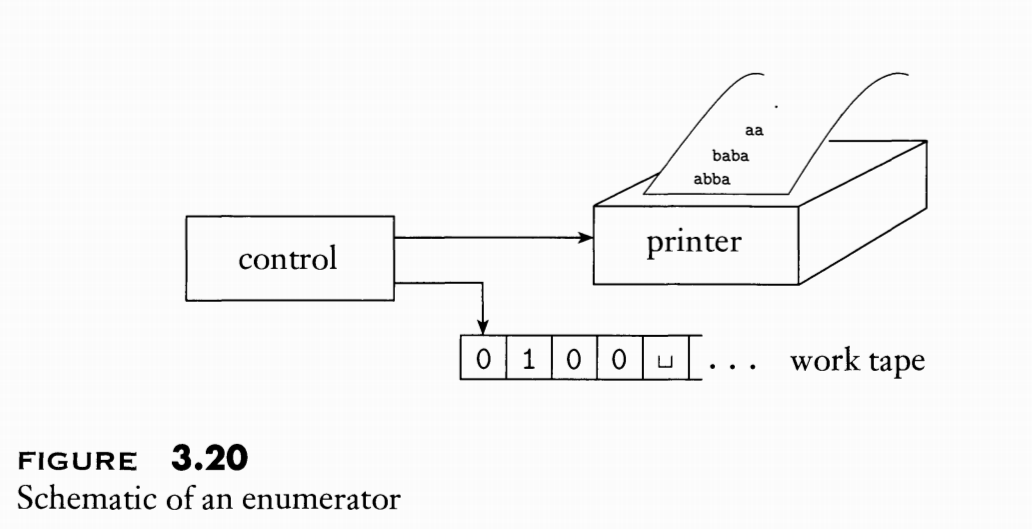
\includegraphics[scale=0.47]{images/figure320.png}
\end{center}
An enumerator E starts with a blank input tape. If the enumerator doesn’t
halt, it may print an infinite list of strings. The language enumerated by $E$
is the collection of all the strings that it eventually prints out. Moreover, $E$
may generate the strings of the language in any order, possibly with repetitions.
Now we are ready to develop the connection between enumerators and Turing-recognizable languages. 

\par\rule{\textwidth}{0.4pt}
\textbf{THEOREM 3.2} \textit{A language is Turing-recognizable if and only if some enumerator enumerates it.}
\par\textbf{PROOF}
First we show that if we have an enumerator $E$ that enumerates a language $A$, a TM $M$ recognizes $A$. The $TM$ M works in the following way.
$M$ = “On input $w$:
\begin{enumerate}[label=\textbf{\arabic*}]
    \item Run $E$. Every time that $E$ outputs a string, compare it with $w$.
    \item If $w$ ever appears in the output of $E$, accept"
\end{enumerate}

Clearly, $M$ accepts those strings that appear on $E$’s list.
Now we do the other direction. If TM $M$ recognizes a language $A$, we can
construct the following enumerator $E$ for $A$. Say that $s_1, s_2, s_3, ...$ is
a list of all possible strings in $\sum$*.
\par$E$ = "Ignore the input.
\begin{enumerate}[label=\textbf{\arabic*}]
    \item Repeat the following for $i = 1, 2, 3, ...$.
    \item Run $M$ for $i$ steps on each input.  $s_1, s_2, ..., s_i$
    \item If any computations accept, print out the corresponding $s_j$.”
\end{enumerate}
If $M$ accepts a particular string $s$, eventually it will appear on the list generated
by $E$. In fact, it will appear on the list infinitely many times because $M$ runs
from the beginning on each string for each repetition of step 1. This procedure
gives the effect of running $M$ in parallel on all possible input strings. 
\subsection{Define the notion of multitape Turing machine. Prove that every multitape Turing machine has an equivalent single tape Turing machine}
\emph{cf Sipser, pp. 148}
\par A multitape Turing machine is like an ordinary Turing machine with several
tapes. Each tape has its own head for reading and writing. Initially the input
appears on tape 1, and the others start out blank. The transition function is
changed to allow for reading, writing, and moving the heads on some or all of
the tapes simultaneously. Formally, it is \todo[inline]{add equation}
where $k$ is the number of tapes. The expression 
\todo[inline]{add equation}

means that, if the machine is in state $q_i$ and heads 1 through $k$ are reading symbols $a_1$ through $a_k$, the machine goes to state $q_j$, writes symbols $b_1$ through $b_k$,
and directs each head to move left or right, or to stay put, as specified.
Multitape Turing machines appear to be more powerful than ordinary Turing
machines, but we can show that they are equivalent in power. Recall that two
machines are equivalent if they recognize the same language. 
\par\rule{\textwidth}{0.4pt}
\textbf{THEOREM 3.13} \textit{Every multitape Turing machine has an equivalent single-tape Turing machine.}
\par\textbf{PROOF} We show how to convert a multitape TM $M$ to an equivalent singletape TM $S$. The key idea is to show how to simulate $M$ with $S$.
Say that $M$ has $k$ tapes. Then $S$ simulates the effect of $k$ tapes by storing
their information on its single tape. It uses the new symbol \# as a delimiter to
separate the contents of the different tapes. In addition to the contents of these
tapes, $S$ must keep track of the locations of the heads. It does so by writing a tape
symbol with a dot above it to mark the place where the head on that tape would
be. Think of these as “virtual” tapes and heads. As before, the “dotted” tape
symbols are simply new symbols that have been added to the tape alphabet.\\
The following figure illustrates how one tape can be used to represent three tapes. 
\begin{center}
    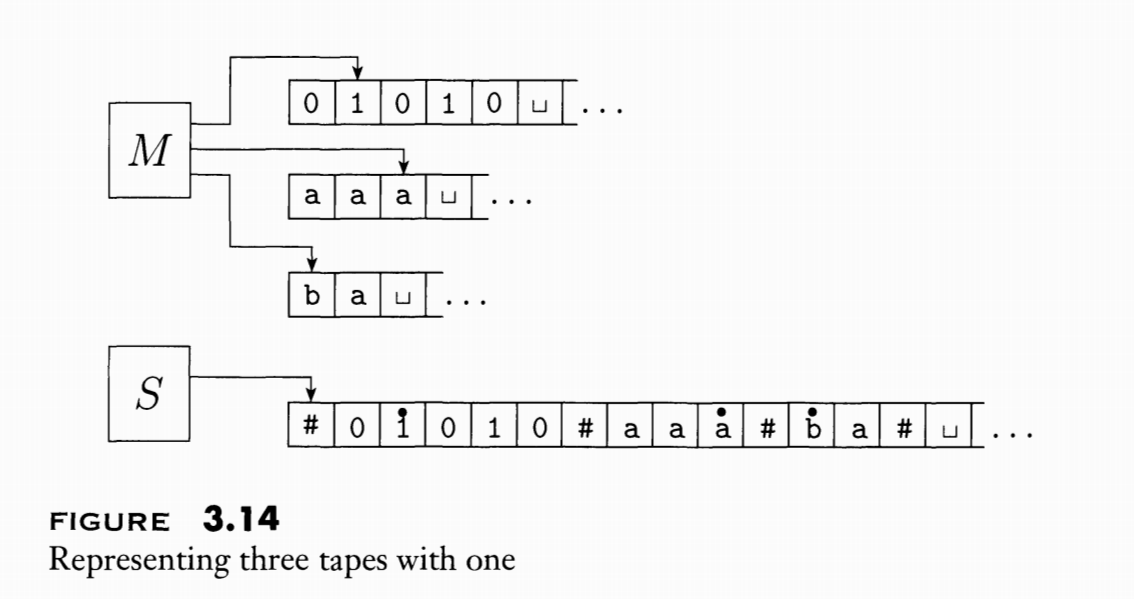
\includegraphics[scale=0.47]{images/figure314.png}
\end{center}
$S$ = "On input $w = w_1, ..., w_n$ :
\begin{enumerate}[label=\textbf{\arabic*}]
    \item Firsts $S$ puts its tape into the format that represent all $k$ tapes of $M$. The formatted tape contains \todo[inline]{Add equation}
    \item To simulate a single move, $S$ scans its tape $t$ from the first \#, which marks the left-hand end, to the $(k+1)$st \#, which marks the right-hand end, in order to determine the symbols under the virtual heads. Then $S$ makes a second pass to update the tapes according to the way that $M$'s transition function dictates. 
    \item If at any point $S$ moves one of the virtual heads to the right onto $a$ \#, this action signifies that M has moved the corresponding head onto the previously unread blank portion of that tape. So $S$ writes a blank symbol on this tape cell and shifts the tape contents, from this cell until the rightmost $\#$, one unit to the right. Then it continues the simulation as before."
\end{enumerate} 

\subsection{What is the Church-Turing thesis ? Give a list of arguments in favor of this thesis ? Why is it not a theorem}
\emph{cf Sipser, pp. 155}
\par\textbf{HILBERT’S PROBLEMS}
\par In 1900, mathematician David Hilbert delivered a now-famous address at the
International Congress of Mathematicians in Paris. In his lecture, he identified twenty-three mathematical problems and posed them as a challenge for the
coming century. The tenth problem on his list concerned algorithms.
Before describing that problem, let’s briefly discuss polynomials. A polynomial is a sum of terms, where each term is a product of certain variables and a constant called a coefficient. For example, 
\todo[inline]{add equation}
is a term with coefficient 6, and
\todo[inline]{add equation}
is a polynomial with four terms over the variables $x$, $y$ and $z$ For this discussion,
we consider only coefficients that are integers. A root of a polynomial is an
assignment of values to its variables so that the value of the polynomial is 0.
This polynomial has a root at $x = 5$, $y = 3$, and $z = 0$. This root is an integral
root because all the variables are assigned integer values. Some polynomials have
an integral root and some do not. \\
Hilbert’s tenth problem was to devise an algorithm that tests whether a polynomial has an integral root. He did not use the term algorithm but rather
\begin{quoting}[font=itshape, begintext={``}, endtext={''}]
a process according to which it can be determined by a finite number of operations.
\end{quoting}
Interestingly, in the way he phrased this problem, Hilbert explicitly
asked that an algorithm be “devised.” Thus he apparently assumed that such an
algorithm must exist, someone need only find it. \\
As we now know, no algorithm exists for this task; it is algorithmically unsolvable. For mathematicians of that period to come to this conclusion with their
intuitive concept of algorithm would have been virtually impossible. The intuitive concept may have been adequate for giving algorithms for certain tasks, but
it was useless for showing that no algorithm exists for a particular task. Proving
that an algorithm does not exist requires having a clear definition of algorithm.
Progress on the tenth problem had to wait for that definition.
\par \par The \textbf{definition} came in the 1936 papers of Alonzo Church and Alan Turing. Church used a notational system called the $\lambda$-calculus to define algorithms.
Turing did it with his “machines.” These two definitions were shown to be
equivalent. This connection between the informal notion of algorithm and the
precise definition has come to be called the Church-Turing thesis.
The Church-Turing thesis provides the definition of algorithm necessary to
resolve Hilbert’s tenth problem. In 1970, Yuri Matijasevic, building on work of
Martin Davis, Hilary Putnam, and Julia Robinson, showed that no algorithm exists for testing whether a polynomial has integral roots. 
\begin{center}
    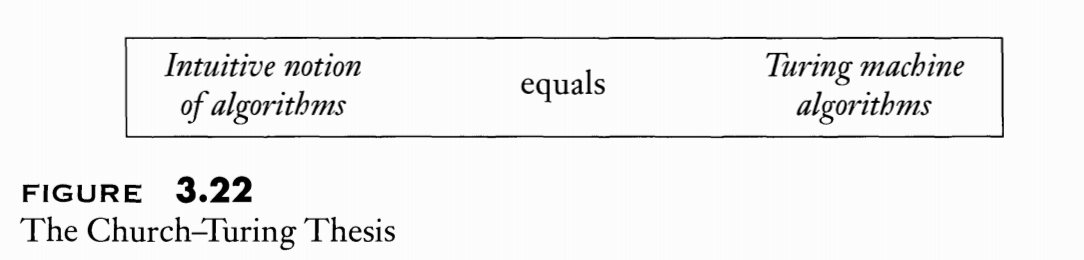
\includegraphics[scale=0.45]{images/figure322.png}
\end{center}
\todo[inline]{Need more info}
\subsection{Why don’t we use the notions of finite automata or context-free grammars to formalize algorithms} 
\emph{cf Sipser, pp. 138}
\par First, here are the differences between a Turing machine and a finite automata : 
\begin{enumerate}
    \item A Turing machine can both write on the tape and read from it.
    \item The read-write head can move both to the left and to the right.
    \item The tape is infinite.
    \item The special states for rejecting and accepting take effect immediately.
\end{enumerate}

\todo[inline]{Not in the book, need research}
\end{document}